% Copyright 2004 by Till Tantau <tantau@users.sourceforge.net>.
%
% In principle, this file can be redistributed and/or modified under
% the terms of the GNU Public License, version 2.
%
% However, this file is supposed to be a template to be modified
% for your own needs. For this reason, if you use this file as a
% template and not specifically distribute it as part of a another
% package/program, I grant the extra permission to freely copy and
% modify this file as you see fit and even to delete this copyright
% notice. 

\documentclass{beamer}
\usepackage{subcaption}

% Comment these 3 lines out for without notes
\usepackage{pgfpages}
\setbeameroption{show notes}
\setbeameroption{show notes on second screen=right}


% There are many different themes available for Beamer. A comprehensive
% list with examples is given here:
% http://deic.uab.es/~iblanes/beamer_gallery/index_by_theme.html
% You can uncomment the themes below if you would like to use a different
% one:
% \usetheme{AnnArbor}
% \usetheme{Antibes}
% \usetheme{Bergen}
% \usetheme{Berkeley}
% \usetheme{Berlin}
% \usetheme{Boadilla}
% \usetheme{boxes}
\usetheme{CambridgeUS}
% \usetheme{Copenhagen}
% \usetheme{Darmstadt}
% \usetheme{default}
% \usetheme{Frankfurt}
% \usetheme{Goettingen}
% \usetheme{Hannover}
% \usetheme{Ilmenau}
% \usetheme{JuanLesPins}
% \usetheme{Luebeck}
% \usetheme{Madrid}
% \usetheme{Malmoe}
% \usetheme{Marburg}
% \usetheme{Montpellier}
% \usetheme{PaloAlto}
% \usetheme{Pittsburgh}
% \usetheme{Rochester}
% \usetheme{Singapore}
% \usetheme{Szeged}
% \usetheme{Warsaw}

\title[3D reconstruction]{3D Reconstruction on an IMU enabled Mobile Device}

% A subtitle is optional and this may be deleted
\subtitle{Summer Undergraduate Research Award - 2015}

\author[Kartikeya \and Prateek]{\hspace{.063\textwidth} Kartikeya Gupta \and Prateek Kumar Verma \\\small CGPA:9.78 \hspace{.1\textwidth} \and \small CGPA:8.87}
% - Give the names in the same order as the appear in the paper.
% - Use the \inst{?} command only if the authors have different
%   affiliation.

\institute[IITD] % (optional, but mostly needed)
{
  Department of Computer Science and Engineering\\
  IIT Delhi
  \and
  Under supervision of \\
  \textbf{Prof. Subhashis Banerjee} \\
  Department of Computer Science and Engineering
}
% - Use the \inst command only if there are several affiliations.
% - Keep it simple, no one is interested in your street address.

\date{March 19, 2015}
% - Either use conference name or its abbreviation.
% - Not really informative to the audience, more for people (including
%   yourself) who are reading the slides online

\subject{Theoretical Computer Science}
% This is only inserted into the PDF information catalog. Can be left
% out. 

% If you have a file called "university-logo-filename.xxx", where xxx
% is a graphic format that can be processed by latex or pdflatex,
% resp., then you can add a logo as follows:

% \pgfdeclareimage[height=0.5cm]{university-logo}{university-logo-filename}
% \logo{\pgfuseimage{university-logo}}

% Delete this, if you do not want the table of contents to pop up at
% the beginning of each subsection:
\AtBeginSubsection[]
{
  % \begin{frame}<beamer>{Outline}
  %   \tableofcontents[currentsection,currentsubsection]
  % \end{frame}
}

% Let's get started
\begin{document}

\begin{frame}
  \titlepage
\end{frame}

% \begin{frame}{Outline}
  % \tableofcontents
  % You might wish to add the option [pausesections]
% \end{frame}

% Section and subsections will appear in the presentation overview
% and table of contents.
% \section{First Main Section}

% \subsection{First Subsection}

\begin{frame}{Objectives}{}
  % \begin{itemize}
  % \item {
  %   My first point.
  % }
  % \item {
  %   My second point.
  % }
  % \end{itemize}
  3D reconstruction on an IMU enabled mobile device.
\end{frame}

\begin{frame}{What is 3D reconstruction?}{}
    \begin{figure}[ht!]
      \centering
      \begin{subfigure}{.5\textwidth}
          \centering
          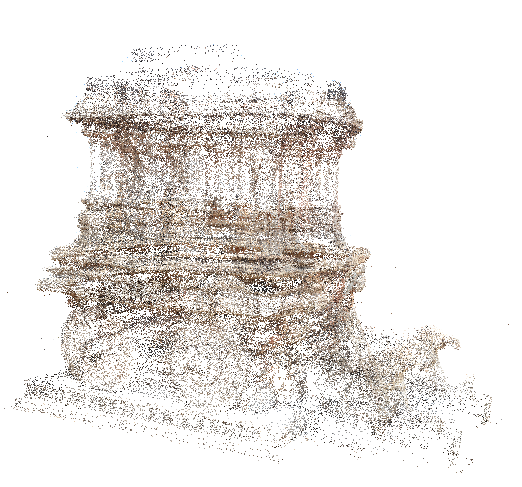
\includegraphics[width=1.0\linewidth]{sparse_chariot.png}
          \caption{Sparse reconstruction}
          \label{fig:sub1}
      \end{subfigure}%
      \begin{subfigure}{.5\textwidth}
          \centering
          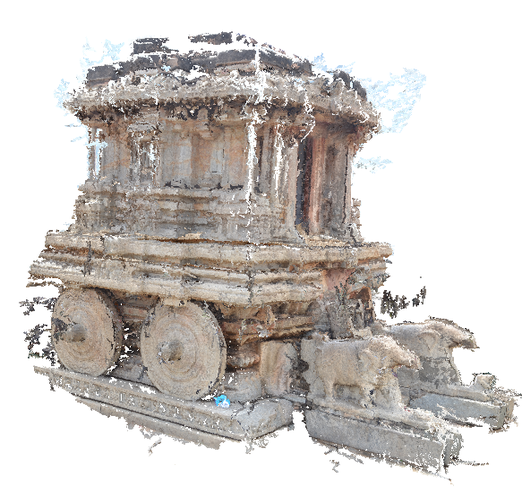
\includegraphics[width=1.0\linewidth]{dense_chariot.png}
          \caption{Dense reconstruction}
          \label{fig:sub2}
      \end{subfigure}
      % \caption{3D reconstruction}
      \label{figstart}
    \end{figure}
    \note{\textcolor{red}{Kartikeya\\}}
    \note{Tell about sparse reconstruction\\}
    \note{\textcolor{green}{Prateek\\}}
    \note{Tell about dense reconstruction\\}
\end{frame}

\begin{frame}{Why 3D reconstruction?}{}
    \begin{itemize}
      \item Generation of a 3D printable file allowing engineers and students to analyse an object more closely
      \item Field of medical science 
      \item Archaeological application
      \item Localization of tourist sites
    \end{itemize}
    \note{\textcolor{red}{Kartikeya\\}}
    \note{chill.\\}
    \note{\textcolor{green}{Prateek\\}}
    \note{Elaborate on each.\\}
\end{frame}


% \subsection{Present Pipeline}

\begin{frame}{3D reconstruction method}{Intrinsic Camera Parameters}
  \begin{itemize} 
    \item Internal calibration matrix  $K$ is internal to the camera itself and is defined in terms of the  camera focal length $f$ and the principal points $c_x$ and  $c_y$ defined as image centers in pixels.
  \begin{equation}
   \mathbf{K}  = 
    \begin{bmatrix}
    f & 0 & c_x \\ 0 & f & c_y \\
    0 & 0 & 1 
    \end{bmatrix}
  \end{equation}
  \end{itemize}
  \note{\textcolor{green}{Prateek\\}}
  \note{Speak about internal camera parameters}
\end{frame}

\begin{frame}{3D reconstruction method}{Extrinsic Camera Parameters}
 \begin{itemize}
  \item External calibration matrix $[R|\textbf{t}]$ constitute the rigid transformations viz. the rotation and translation between the camera coordinate system and the world coordinate system.
  \begin{figure}
    \centering
    %\begin{tabular}{ccc}
    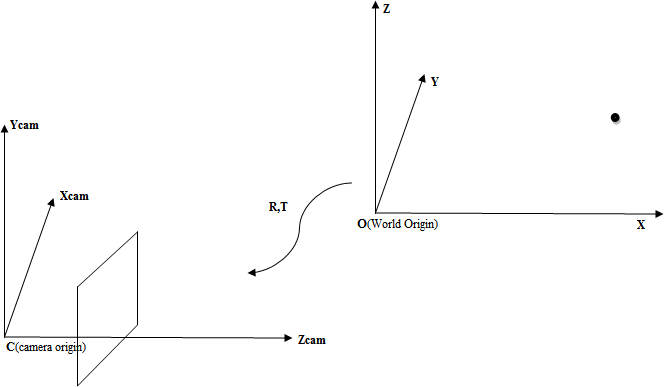
\includegraphics[width=0.3\textwidth]{CameraWorld.png}
    \caption{External calibration}
    %\end{tabular}
  \end{figure}
  \item Together they form the projection matrix $P$
  \begin{equation*}
    P = K[R|\textbf{t}]
    \end{equation*}
    s.t. \begin{equation*} \mathbf{x} = P\mathbf{X} \end{equation*}
  \end{itemize}
  \note{\textcolor{red}{Kartikeya\\}}
  \note{Speak about extrinsic camera parameters}
\end{frame}

\begin{frame}{3D reconstruction method}{Stereo Correspondence Generation}
  \begin{itemize}
    \item Use image descriptors like SIFT for finding set of matching feature points $\mathbf{x}'$ and $\mathbf{x}$ in between a pair of images.
  \begin{figure}[ht!]
    \centering
    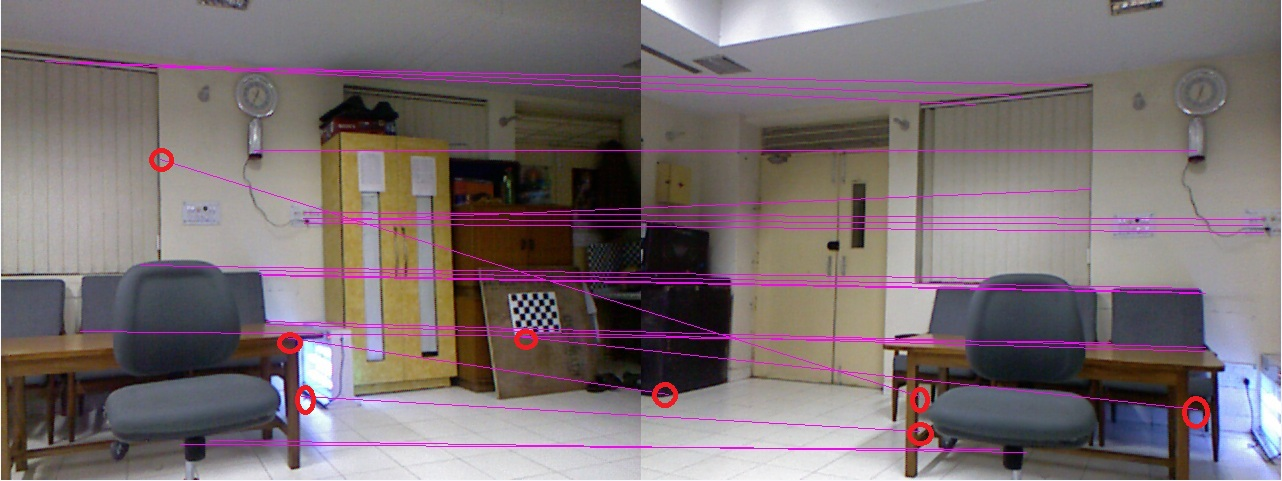
\includegraphics[width=\linewidth]{siftcorres.jpg}
    % \caption{Accuracy of accelerometer data across different devices (scale cm)\label{fig1}}
  \end{figure}
    \item Lots of false matches
  \end{itemize}
  \note{\textcolor{red}{Kartikeya\\}}
  \note{speak about the false matches that are taking place which need to be removed}
\end{frame}

\begin{frame}{3D reconstruction method}{Triangulation}
  \begin{figure}[ht!]
    \centering
    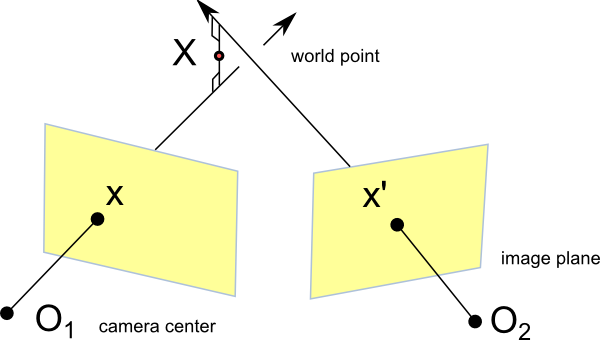
\includegraphics[width=0.6\linewidth]{triangulation.png}
    % \caption{Accuracy of accelerometer data across different devices (scale cm)\label{fig1}}
  \note{\textcolor{green}{Prateek\\}}
  \note{About triangulation and pairwise image correspondence}

  \end{figure}
\end{frame}

\begin{frame}{3D reconstruction method}{Present Pipeline}
  \begin{figure}[ht!]
    \centering
    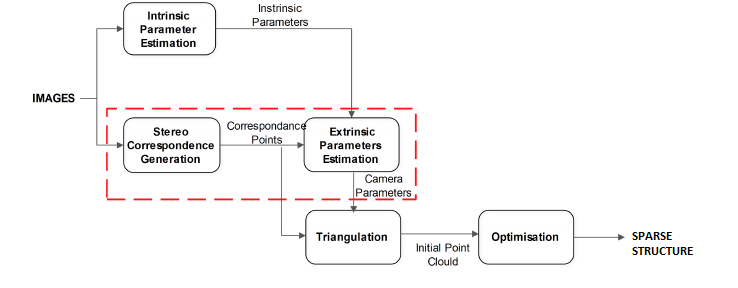
\includegraphics[width=\linewidth]{traditional_paipeline.png}
    % \caption{Accuracy of accelerometer data across different devices (scale cm)\label{fig1}}
  \end{figure}
  \note{\textcolor{red}{Kartikeya\\}}
  \note{Explain about the expensive red box}
\end{frame}

\begin{frame}{Proposed Framework}{}
  \begin{figure}[ht!]
    \centering
    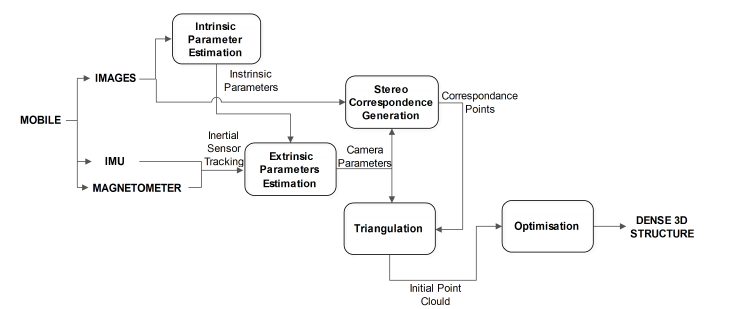
\includegraphics[width=\linewidth]{our_pipeline.png}
    % \caption{Accuracy of accelerometer data across different devices (scale cm)\label{fig1}}
  \end{figure}
  \note{\textcolor{green}{Prateek\\}}
  \note{Explain about the entire framework and how this is better than earlier}

\end{frame}

\begin{frame}{Phases of the Project}{1) Position and structure estimation}
  \begin{enumerate}
        \item Smoothening the raw sensor output data.
        \item Incorporating gyroscope reading to reduce drift.
        \item Using the camera feed to obtain displacement and orientation from visual tracking.
  \end{enumerate}
  \note{\textcolor{green}{Prateek\\}}
  \note{Give an overview about the part}

\end{frame}
\begin{frame}{Phases of the Project}{2) 3D Reconstruction}
  \begin{enumerate}
        \item Obtain sparse 3D reconstruction based on camera parameters obtained previously.
        \item Use tracking methods for dense correspondence of points.
        \item Use guided matching by indirect computation of fundamental matrix from estimated camera motion from sensor data to enrich the correspondences.
        \item Triangulate dense correspondences and do global refinement. 
      \end{enumerate}
  \note{\textcolor{red}{Kartikeya\\}}
  \note{Give an explanation about the 3d reconstruction part}
\end{frame}

\begin{frame}{Our experience so far}{}
    \begin{figure}[ht!]
      \centering
      \begin{subfigure}{.5\textwidth}
          \centering
          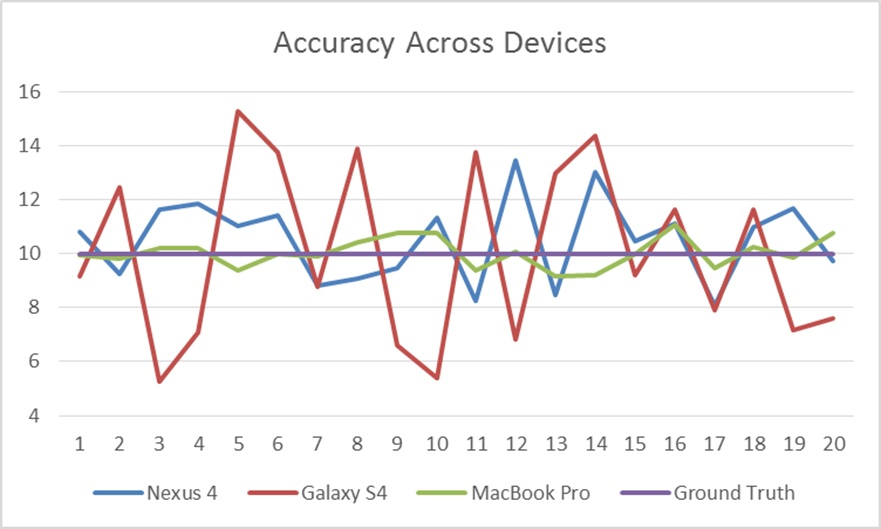
\includegraphics[width=1.0\linewidth]{graph.jpg}
          \caption{Accuracy of accelerometer data across different devices (scale cm)}
          % \label{fig:sub1}
      \end{subfigure}%
      \begin{subfigure}{.5\textwidth}
          \centering
          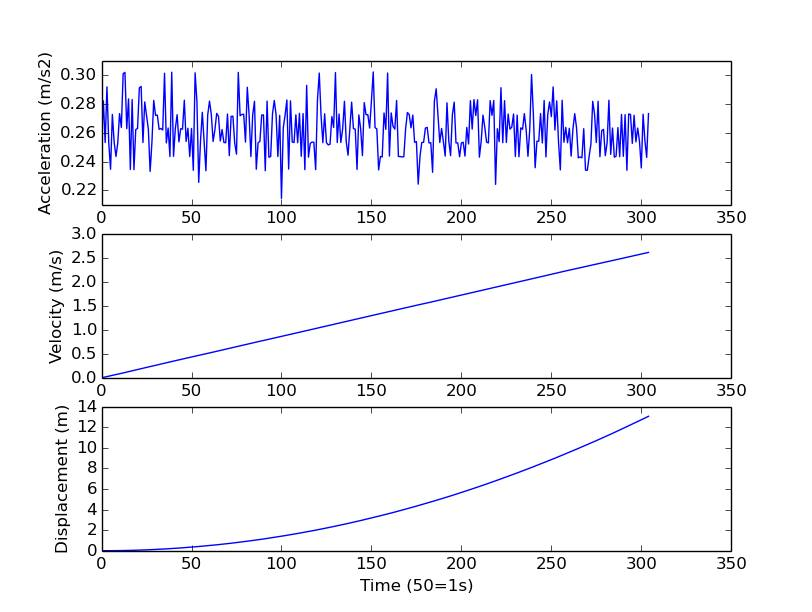
\includegraphics[width=1.0\linewidth]{integration.jpg}
          \caption{Obtaining velocity and displacement from static accelerometer data}
          % \label{fig:sub2}
      \end{subfigure}
      % \caption{3D reconstruction}
      % \label{figstart}
    \end{figure}
    \note{\textcolor{red}{Kartikeya\\}}
    \note{Explain figure 1\\
          3 devices taken, for 20 readings each ad the distance calculated is plotted.\\
          The accuracy can be seen, macbook pro gives the best accuracy followed by nexus and then S4\\}
    \note{\textcolor{green}{Prateek\\}}
    \note{Explain figure 2\\
          }
\end{frame}



\begin{frame}{}{}
  \begin{figure}[ht!]
    \centering
    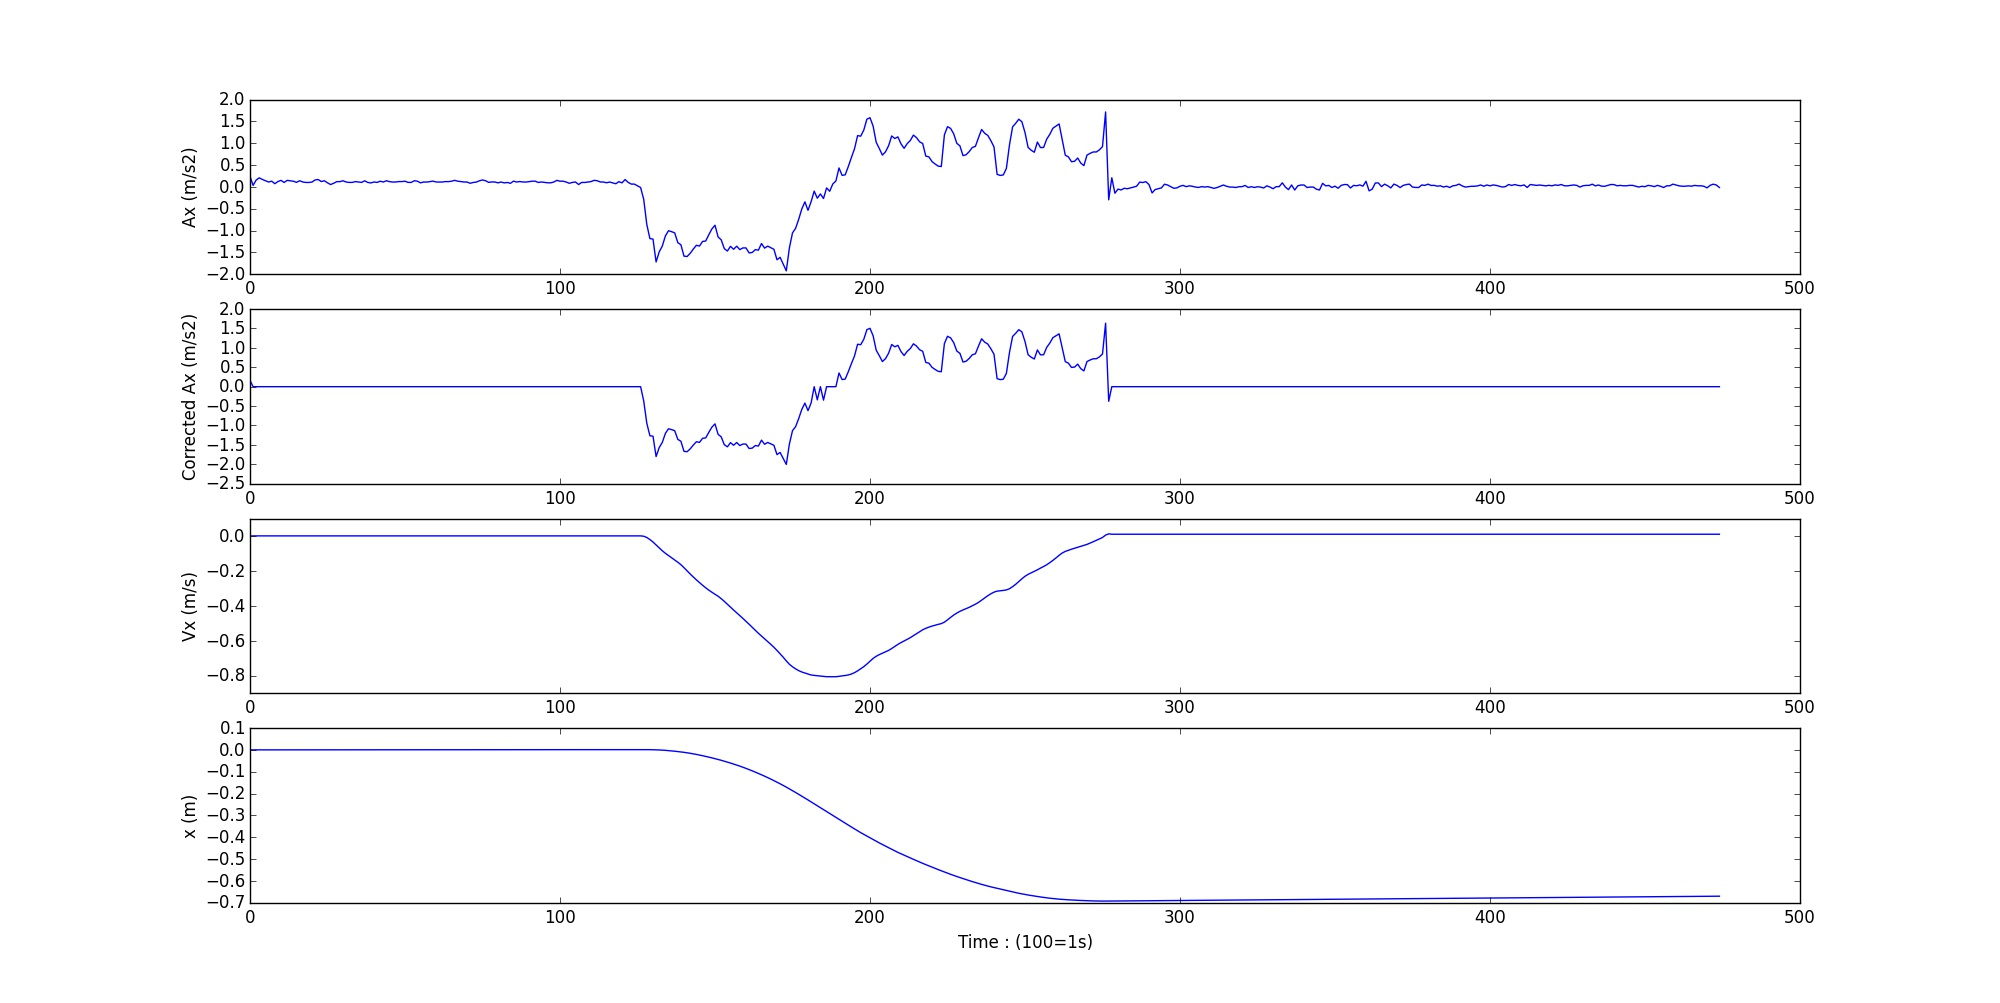
\includegraphics[width=\linewidth]{Corrected.jpeg}
    \caption{Applying smoothening techniques}
  \end{figure}
  \note{\textcolor{red}{Kartikeya\\}}
  \note{Explain about the smoothening taking place, static bias removal and drift correction }
\end{frame}

% \begin{frame}{More Applications}{}
%   \begin{itemize}
%     \item Quick 3D printable file
%     \item Field of medical science
%     \item Archaeological application
%     \item Localization of tourist sites
%   \end{itemize}
%   \note{\textcolor{green}{Prateek\\}}
%   % \note{Fundae pel :P}
% \end{frame}


\begin{frame}{Future Possibilites}{}
    \begin{itemize}
      \item Improving the algorithm for a quicker and more efficient 3D recon-
struction.
      \item Releasing applications for Apple, Android and Windows platforms
for near real time 3D reconstruction on the device itself.
      \item Getting a more detailed texture mapping of the object.
      \item Making an object recognition software on the basis of this 3D recon-
struction.
    \end{itemize}
    \note{\textcolor{red}{Kartikeya\\}}
    \note{explain first two}
    \note{\textcolor{green}{Prateej\\}}
    \note{explain last two}
\end{frame}


\begin{frame}{Budget}{}
\begin{block}{Budget}
Rs. 25000 to purchase an android smart phone having high quality sensors and a high resolution camera.
\end{block}
  \note{\textcolor{red}{Kartikeya\\}}
\end{frame}


\begin{frame}
\vfill
\begin{center}
\huge{Thank You}
\end{center}
\vfill
\note{MISSION ACCOMPLISHED}
\end{frame}

% % You can reveal the parts of a slide one at a time
% % with the \pause command:
% \begin{frame}{Second Slide Title}
%   \begin{itemize}
%   \item {
%     First item.
%     \pause % The slide will pause after showing the first item
%   }
%   \item {   
%     Second item.
%   }
%   % You can also specify when the content should appear
%   % by using <n->:
%   \item<3-> {
%     Third item.
%   }
%   \item<4-> {
%     Fourth item.
%   }
%   % or you can use the \uncover command to reveal general
%   % content (not just \items):
%   \item<5-> {
%     Fifth item. \uncover<6->{Extra text in the fifth item.}
%   }
%   \end{itemize}
% \end{frame}

% \section{Second Main Section}

% \subsection{Another Subsection}

% \begin{frame}{Blocks}
% \begin{block}{Block Title}
% You can also highlight sections of your presentation in a block, with it's own title
% \end{block}
% \begin{theorem}
% There are separate environments for theorems, examples, definitions and proofs.
% \end{theorem}
% \begin{example}
% Here is an example of an example block.
% \end{example}
% \end{frame}

% % Placing a * after \section means it will not show in the
% % outline or table of contents.
% \section*{Summary}

% \begin{frame}{Summary}
%   \begin{itemize}
%   \item
%     The \alert{first main message} of your talk in one or two lines.
%   \item
%     The \alert{second main message} of your talk in one or two lines.
%   \item
%     Perhaps a \alert{third message}, but not more than that.
%   \end{itemize}
  
%   \begin{itemize}
%   \item
%     Outlook
%     \begin{itemize}
%     \item
%       Something you haven't solved.
%     \item
%       Something else you haven't solved.
%     \end{itemize}
%   \end{itemize}
% \end{frame}



% % All of the following is optional and typically not needed. 
% \appendix
% \section<presentation>*{\appendixname}
% \subsection<presentation>*{For Further Reading}

% \begin{frame}[allowframebreaks]
%   \frametitle<presentation>{For Further Reading}
    
%   \begin{thebibliography}{10}
    
%   \beamertemplatebookbibitems
%   % Start with overview books.

%   \bibitem{Author1990}
%     A.~Author.
%     \newblock {\em Handbook of Everything}.
%     \newblock Some Press, 1990.
 
    
%   \beamertemplatearticlebibitems
%   % Followed by interesting articles. Keep the list short. 

%   \bibitem{Someone2000}
%     S.~Someone.
%     \newblock On this and that.
%     \newblock {\em Journal of This and That}, 2(1):50--100,
%     2000.
%   \end{thebibliography}
% \end{frame}

\end{document}


